\chapter{Literature Review}
\label{cha:literature-review}

In the previous chapter, we gave a detailed definition of cellular 
automata, neural networks, and reservoir computing, and described the interplay 
between them. The current chapter aims to 
provide an overview of several fields associated with learning and complex
systems that have informed and influenced our work in this thesis. We begin by reviewing related
work on complexity measures for dynamical and complex systems (Section
\ref{sec:measuring-complexity}). We also review works on defining and
understanding emergence (Section \ref{sec:emergence}), evolutionary methods for
searching solutions in complex spaces (Section \ref{sec:evol-algor}), methods
for constructing open-ended evolving systems (Section
\ref{sec:open-ended-evolution-1}), and methods for extracting and using the
computations happening within complex systems (Section
\ref{sec:comp-with-compl}).

\section{Measuring complexity\label{sec:measuring-complexity}}

Measuring the complexity of a system is a fundamentally difficult task. Many
complex systems exhibit what Peter Grassberger calls \emph{self-generated
  complexity} \parencite{grassbergerQuantitativeTheorySelfgenerated1986}. This
means that the formulation of the system is translationally invariant and the
observed structure arises from a spontaneous breakdown of translational
invariance. For example, \ac{CA} has a uniform update rule, but the complexity 
arises locally in some of them. Unfortunately, there is no universally accepted and formalized notion
of ``complexity'', although most intuitively agree that it exists. For
example, Figure \ref{fig:three_eca_complex} shows three examples of behaviors
generated by 1D \acp{ECA}. Most people would consider the leftmost figure
\ref{fig:simple} to be not complex. However, depending on one's definition of
complexity, the last picture could be labeled as complex.

\begin{figure}[htbp]
  \centering
   \begin{subfigure}[b]{.03\linewidth}
    \centering
    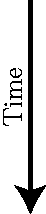
\includegraphics[width=\linewidth]{figures/arrow.pdf}
    \caption*{}
  \end{subfigure}
  \begin{subfigure}[b]{.31\linewidth}
    \centering
    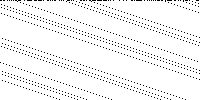
\includegraphics[width=\linewidth]{figures/three_simple_eca.png}
    \caption{}
   \label{fig:simple}
  \end{subfigure}
  \begin{subfigure}[b]{.31\linewidth}
    \centering
    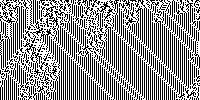
\includegraphics[width=\linewidth]{figures/three_complex_eca.png}
    \caption{}
   \label{fig:complex}
  \end{subfigure}
  \begin{subfigure}[b]{.31\linewidth}
    \centering
    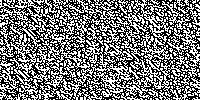
\includegraphics[width=\linewidth]{figures/three_random_eca.png}
    \caption{}
   \label{fig:random}
  \end{subfigure}
  \caption{Three 1D \aclp{CA} with qualitatively different behavior. The left
    (\ref{fig:simple}) and right (\ref{fig:random}) \acp{CA} are usually not
    defined as ``complex'', whereas the middle \ac{CA} (\ref{fig:complex})
    appears to be more complex than the others. The Figures show \acp{CA} space-time 
    diagrams. Each row represents the state of the \ac{CA} at a single time step, with 
    the time increasing from top to bottom.}
  \label{fig:three_eca_complex}
\end{figure}

\begin{figure}[htbp]
  \centering
  \scalebox{1}{
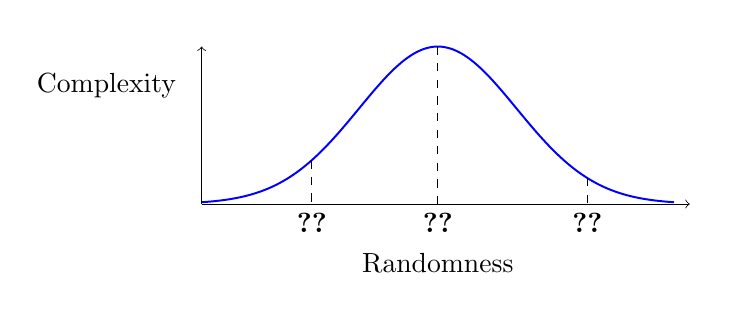
\begin{tikzpicture}
% define normal distribution function 'normaltwo'
\def\normaltwo{\x,{2*1/exp(((\x-3)^2)/2)}}

% input y parameter
\def\ya{4.9}
\def\fya{2*1/exp(((\ya-3)^2)/2)}

\def\yb{1.4}
\def\fyb{2*1/exp(((\yb-3)^2)/2)}

\def\yc{3}
\def\fyc{2*1/exp(((\yc-3)^2)/2)}

% Draw and label normal distribution function
\draw[color=blue,domain=0:6,smooth,samples=50, line width=0.25mm] plot (\normaltwo) node[right] {};

% Add dashed line dropping down from normal.
\draw[dashed] ({\ya},{\fya}) -- ({\ya},0) node[below] {\ref{fig:random}};
\draw[dashed] ({\yb},{\fyb}) -- ({\yb},0) node[below] {\ref{fig:simple}};
\draw[dashed] ({\yc},{\fyc}) -- ({\yc},0) node[below] {\ref{fig:complex}};


% Add axis labels
\draw (-.2,1.5) node[left] {Complexity};
\draw (3,-.5) node[below] {Randomness};

% Add axes
\draw[->,line width=0.1mm] (0,0) -- (6.2,0) node[right] {};
\draw[->,line width=0.1mm] (0,0) -- (0,2) node[above] {};

\end{tikzpicture}}
\caption{\emph{Ideal} ``complexity'' curve as a function of the ``randomness''
  of a system. The three \acp{CA} from figure \ref{fig:three_eca_complex} are
  displayed at their approximate expected location on that curve. This curve is
  just for illustrative purposes and does not correspond to any true function
  linking randomness and complexity.}
\label{fig:complexity_curve}
\end{figure}

No clear observables quantities and protocols have been proposed that would give a
quantitative notion of complexity.
\textcite{grassbergerProblemsQuantifyingSelfgenerated1989} argued that no single
quantity is sufficient to measure complexity since it depends on exactly how the
meaning is assigned to this term. Even when some meaning has been fixed by the
definition of an observable quantity, the statistics of the measurement of this
observable are also crucial to its
interpretation~\parencite{gutowitzCellularAutomataSciences1995}.

Despite these drawbacks, we seek a measure of complexity that matches intuition
as well as possible. Such a measure would assign low complexity to both simple
objects and random objects and high complexity to objects in between. For
illustration, we place the three \acp{ECA} from Figure
\ref{fig:three_eca_complex} on this ideal complexity curve, shown in Figure
\ref{fig:complexity_curve}. For example, in Chapter \ref{cha:meas-compl-evolv},
we develop a complexity metric that matches the human intuition of complexity on a
dataset of cellular automata.

One of the most widely known concepts of the complexity of symbol
sequences, ``algorithmic complexity,'' should also be called a measure of
information. This is the position held by one of its co-creators
\parencite{chaitinInformationRandomnessIncompleteness1990}. In the literature,
information measures are often used as complexity metrics. These quantities
are better measures of ``randomness'' than complexity, but they are nonetheless
important for the study of complex systems. In this section, we list several
complexity measures, including information measures that have influenced our
research.

\subsection{Information content}
For an event $E$ with probability $P$, the information content of this event is
defined as the negative logarithm of its probability, that is,

\begin{equation}
  I(E) :=  -\log(P).
\end{equation}

This metric quantifies how unlikely an event is and depends on how the
probability $P$ was estimated in practice. This notion is at the foundation of
information theory. The information content of a finite set of $N$ events is maximal 
when all events are equally probable, that is $I(E) = \log(N)$.

\subsection{Shannon Entropy}
Shannon entropy is defined as the expected information content of the input
\parencite{shannonMathematicalTheoryCommunication1975}. We have

\begin{align*}
  H(X) := \mathbb{E}[-\log(P(X))].
\end{align*}

This measure is a lower bound on the number of bits that the input could be
compressed to.

In the case of a 1D \ac{ECA}, the Shannon entropy could be computed cell-wise
over the time distribution of the states, producing an entropy per cell score
that can be averaged over an entire automaton. This measure is, for example, one
of the measures used by Wolfram in
\parencite{wolframStatisticalMechanicsCellular1983} and by Langton in
\parencite{langtonComputationEdgeChaos1990} to study how the parameter $\lambda$
affects the behavior of the automaton. There are several ways to compute it when
dealing with a CA, depending on which part of the CA is considered as the main
random variable. If the CA is finite, the state at timestep $t$ can be seen as a
random variable that can take one of $2^N$ possible values (with $N$ the width
of the automaton state). In that case, the probability of a state can easily be
estimated by counting its number of occurrences during evolution. For too large
state spaces, this becomes challenging, as it is very unlikely that a given state will
be seen again.

\subsection{Rényi Entropy}
The Rényi entropy is a generalization of Shannon entropy that gives different
weights to events of various probabilities
\parencite{renyiMeasuresEntropyInformation1961}. It is formally defined for an
$\alpha \geq 0, \alpha \neq 1$ and a random variable $X$ with possible outcomes $0, 1, ..., n$ as
\begin{align*}
  H_\alpha(X) = \frac{1}{1-\alpha} \log\left(\sum_{i=0}^np_i^\alpha\right).
\end{align*}

In the limit $\alpha \rightarrow 1$ it is equal to the Shannon entropy, where the probabilities of each event are equally important. $\alpha \rightarrow \infty$ yields the Min-entropy, and we have
$H_{\infty} (X) = \min_{i}(\log(p_{i}))$. With $\alpha \rightarrow 0$ Rényi entropy is the same as
Max-entropy, or topological entropy. Rényi entropy was used by
\textcite{wolframStatisticalMechanicsCellular1983} and
\textcite{lindgrenComplexityMeasuresCellular1988} to estimate the complexity in
infinite \acp{CA}.

\subsection{Mutual information}
The mutual information is a measure of the dependence between two variables. Two
independent variables will have mutual information of zero. If the two are
strongly dependent, for example, if one is a function of another, the mutual
information between them will be larger.

\textcite{chaitinMathematicalDefinitionLife1987} proposes to split a system into
fixed blocks and calculate mutual information among its components.
He uses the maximum value of the mutual information in all possible partitions
to define "life" in a mathematical way. \textcite{shawDrippingFaucetModel1984}
and \textcite{grassbergerQuantitativeTheorySelfgenerated1986} also use the
mutual information measure between two semi-infinite blocks in a sequence to
define complexity. Mutual information has also been used to study the
complexity of \acp{CA} as the parameter $\lambda$ is changed (for details
on $\lambda$ in the context of \ac{CA}, see section \ref{sec:langtons-lambda})
\parencite{gutowitzMethodsDesigningCellular1988,
  liTransitionPhenomenaCellular1990}.


\subsection{Computational complexity}
Algorithms can be described by their space and time complexity, which
respectively correspond to the amount of memory storage and CPU time necessary
to run them \parencite{traubInformationUncertaintyComplexity1983,
  packelRecentDevelopmentsInformationbased1987,
  hopcroftIntroductionAutomataTheory2007}. Algorithms that depend on a parameter
$N$ will be said to be NP-hard if the time needed to run them increases
exponentially with the parameter $N$. NP-hard algorithms can be said to be
complex as they require a supposedly irreducible amount of computation to
compute their output. In practice, this description only applies to computations
that were generated by a hand-designed algorithm and not the kind of
computations self-generated by a complex system that we are interested in. For
example, the computations generated by one \ac{CA} cannot be said to be
computationally more complex than those of another \ac{CA} because the algorithm that
implements them is fundamentally the same and computationally simple. The
computational complexity of an algorithm performed by a dynamical system thus
cannot be effectively used as a measure of the complexity of that system.

\subsection{Solomonoff–Kolmogorov-Chaitin complexity (algorithmic
  complexity)}\label{sec:algo-complexity}

Introduced by Solomonoff \parencite{solomonoffPreliminaryReportGeneral1960},
Kolmogorov \parencite{kolmogorovThreeApproachesQuantitative1968} and Chaitin
\parencite{chaitinLengthProgramsComputing1969,
  chaitinAlgorithmicInformationTheory1977,
  chaitinInformationRandomnessIncompleteness1990}, this complexity measure is
defined for a string $s$ of characters and a universal description language (\eg
a programming language) as the length of the shortest program that can generate
the string $s$.

This number $K(s)$ is called the minimum description length of
$s$. We note that Chaitin prefers to call his field "algorithmic information
theory." His position is that "algorithmic complexity" is a measure of
randomness rather than a measure of complexity
\parencite{chaitinInformationRandomnessIncompleteness1990}.

From the invariance theorem \parencite{solomonoffFormalTheoryInductive1964,
  solomonoffFormalTheoryInductive1964a,
  kolmogorovThreeApproachesQuantitative1968,
  chaitinLengthProgramsComputing1969}, the difference in algorithmic complexity
of the same string $s$ in two different description languages is bounded,
although this bound might be very large in practice.

The algorithmic complexity is uncomputable
\parencite{solomonoffFormalTheoryInductive1964,
  kolmogorovThreeApproachesQuantitative1968}, and there exists strings of
arbitrarily large complexity, which makes it hopeless to use this exact measure
in practice. It can be approximated from above, but no accuracy guarantee can be
given, and the runtime of the approximators can grow arbitrarily large.
Moreover, algorithmic complexity tells us how much information is required to
encode a number, but does not tell us how difficult it is to recreate the number
from that code \parencite{gell-mannSimplicityComplexityDescription1988}.

A range of resource-bounded approximations of algorithmic complexity were
developed to obtain computable complexity measures
\parencite{daleyMinimalprogramComplexitySequences1973,
  daleyInferenceOptimalDescriptions1977,
  ,federUniversalPredictionIndividual1992, koNotionInfinitePseudorandom1986,
  schmidhuberSpeedPriorNew2002}. One rather straightforward way of approaching
the algorithmic complexity of an arbitrary string is to use a compression
algorithm and use the length of the decompression program plus the length of
the compressed string as an upper bound to the algorithmic complexity. This is
similar to the optimal symbol compression ratio (OSCR) algorithm proposed by
\parencite{evansNewUniversalTwo2003}.
\textcite{zenilCompressionBasedInvestigationDynamical2010} used the
compression-based method to classify 1D \ac{ECA}. This method, which often
uses the popular LZ algorithm, can be seen as an independent complexity
measure, also closely related to Lempel-Ziv complexity, described in more
detail in the next section ~\ref{subsection:lempel-ziv}.

However, it is worth noting that when a complex system is described by an
algorithm (such as for a \ac{CA}), the algorithmic complexity is also easily
upper bounded by a constant value entirely defined by the algorithm that
simulated the complex system. For example, for a \ac{CA}, the algorithmic
complexity is lower than the size of the rule table of the automaton, its
characteristics (size, boundary conditions, \etc), its initial state, and the number
of simulation steps. This approximation does not inform us about the difference in
complexity between the two \acp{CA}.

\subsection{Lempel-Ziv complexity}\label{subsection:lempel-ziv}
The Lempel-Ziv complexity, as defined in
\parencite{lempelComplexityFiniteSequences1976} is the number of steps in the LZ
algorithm, directly related to the number of repeated substrings in the
input string. The main idea of this algorithm is to scan the input string while
trying to find some repetition of the previous input in the incoming data. This
builds over time a set of basic components called the exhaustive history of the
string, from which the complete string can be constructed. The number of
components in that set is the Lempel-Ziv complexity of that string.

The compressed length method for measuring complexity uses a compression
algorithm to reduce the size of the input. An input with regularities and
repetitive patterns will produce a small output, whereas a completely random
input will be irreducible to a simpler, shorter string.


\subsection{Logical Depth}

Bennett's logical depth is a measure of complexity based on the algorithmic
complexity \parencite{bennettDissipationInformationComputational1988,
  bennettLogicalDepthPhysical1995}. The main difference is that it takes into
account the computation time (or number of steps) along with the length of the
program used to generate the sequence. It is a combination of algorithmic
complexity and computational complexity. For a universal computer $U$, the
logical depth of a string $x$ at a significance level $s$ is defined as

\begin{equation}
  \label{eq:2}
  \min\{T(p): (|p| - |p^{*}| < s ) \wedge (U(p) = x) \},
\end{equation}
which is the least time required to compute it by a $s$-incompressible program,
that is a program $p$ which length is within $s$ symbols from the optimal program
$p^{*}$ of the algorithmic complexity metric.
% \textcite{gutowitzCellularAutomataSciences1995}

\textcite{antunesComputationalDepthConcept2006} considered logical depth to be
one instance of a more general concept: \emph{computational depth}; and proposed
several other variants.

\subsection{Thermodynamic Depth}

The thermodynamic depth, developed by
\textcite{lloydComplexityThermodynamicDepth1988} is another measure of
complexity based on the intuitive notion that complex systems lie somewhere in
the continuum between order and chaos
\parencite{chaitinInformationRandomnessIncompleteness1990,
  ceccattoComplexityHierarchicalSystems1988, deutschQuantumTheoryChurch1985}.
Similar to computational complexity and logical depth, this metric is designed
to be a measure of how the system came to be in its final state. The complexity
corresponds to how difficult it is to put the system together in that state.

By the definition of thermodynamic depth, the average complexity of a state must be
proportional to the Shannon entropy
\parencite{shannonMathematicalTheoryCommunication1975} of the set of
trajectories that the experiment determines can lead to that state. If we write $p_i$ 
the probability of reaching the target state with the $i$-th possible trajectory, we have 

\begin{equation}
  \label{eq:3}
  S = -\left(\sum_{i} p_{i} \log p_{i}\right).
\end{equation}

The measure of complexity of a macroscopic state $s$ of a system that has
reached that state by the i-th possible trajectory is $-k(\log p_{i})$, where
$p_{i}$ is the probability that the system has reached $s$ by the i-th
trajectory, and $k$ is an arbitrary positive constant. The thermodynamic depth of
the state $s$ is defined as

\begin{equation}
  \label{eq:4}
  \mathcal{D}(s) = -k(\log p_{i}).
\end{equation}

The quantity $\mathcal{D}$ can be thought of as the amount of information
required to specify the trajectory that the system has followed to its present
state. The thermodynamic depth of the whole system is then

\begin{equation}
  \label{eq:5}
  \mathcal{D} = \sum_{s}\mathbb{P}(s)D(s),
\end{equation}
where $\mathbb{P}(s)$ is the probability that the system followed the
trajectory $s$.

\textcite{crutchfieldThermodynamicDepthCausal1999} argued that the thermodynamic
depth is a fundamentally flawed structural complexity measure because it relies
on a set of chosen macroscopic states for the system, which are difficult to
choose and need to be defined separately for each system.
\textcite{lloydComplexityThermodynamicDepth1988} does not mention how these states
are supposed to be chosen, nor do any follow-up work, making this complexity
metric difficult to use in practice.

\subsection{Epsilon-machines}

The $\epsilon$-machine is an approach to complexity that seeks to construct a metric
more suitable for physical systems that also addresses some issues of other
existing complexity metrics \parencite{crutchfieldOrderChaos2012}. It is the
result of the field of computational mechanics, an extension of statistical
mechanics that describes not only the statistical properties of a system but
also how it stores information and how it computes
\parencite{crutchfieldInferringStatisticalComplexity1989,
  crutchfieldCalculiEmergenceComputation1994,
  feldmanMeasuresStatisticalComplexity1998, crutchfieldOrderChaos2012}.
Computational mechanics algorithms take as input the time series being analyzed
and output a minimal, optimized model that can reproduce a time series that is
statistically equivalent to the input time series. The size of the model
produces a metric known as statistical complexity. The models are known as
$\epsilon$-machines. Three optimality theorems say that $\epsilon$-machines capture all the
properties of a process
\parencite{crutchfieldInferringStatisticalComplexity1989,
  crutchfieldThermodynamicDepthCausal1999,
  shaliziComputationalMechanicsPattern2001}: prediction: the $\epsilon$-machine is its
optimal predictor; minimality: compared to all other optimal predictors, the
$\epsilon$-machine of a process is its minimal representation; uniqueness: any minimal
optimal predictor is equivalent to the $\epsilon$-machine.

This model has many attractive properties and was successfully applied to study
the symbolic dynamics of chaotic systems
\parencite{crutchfieldCalculiEmergenceComputation1994}, molecular dynamics
\parencite{ryabovComputationalMechanicsMolecular2011}, single-molecule
microscopy \parencite{kellyNewMethodInferring2012}, and the spatiotemporal
complexity of \acp{CA} \parencite{crutchfieldTurbulentPatternBases1993,
  hansonComputationalMechanicsCellular1997,
  shaliziQuantifyingSelfOrganizationOptimal2004}. The main drawback is the
construction of the $\epsilon$-machine itself, for which there is no
general-purpose approach.

\subsection{Sophistication}

Intuitively, \emph{sophistication} is the complexity in a set of strings of which
the string is a ``typical'' member.
\textcite{motaSophisticationRandomnessDeficiency2013} defines sophistication
based on the original definition of \textcite{koppelStructure1988,
  koppelAlmostMachineindependentTheory1991a}. It measures the amount of structural
information contained in a string. It also uses a follow-up result by
\parencite{vitanyiMeaningfulInformation2006} that shows that Koppel's definition
is equivalent to measuring the complexity of a good model for a string up to
low order terms. The definition uses an intermediate quantity called
\emph{discrepancy} that measures how far a set $S$ is from being a good model
of a string $x$.

Formally, the discrepancy $\Delta$ is defined for a string $x$ and a set $S$ that contains $x$ as
\begin{equation}
  \label{eq:6}
  \Delta(x|S) := \log |S| - K(x) + K(S),
\end{equation}
where $K$ is the Solomonoff–Kolmogorov-Chaitin complexity function.

The sophistication of $x$ is defined as the complexity of the simplest model of
$x$ with a limited discrepancy:

\begin{equation}
  \label{eq:7}
  \text{soph}_{c}(x) := \min_{S}\left\{ K(S): \Delta(x|S) \leq c \right\}
\end{equation}
where the significance level $c$ tells us how much discrepancy the set $S$ is allowed to have.

Koppel’s definition of sophistication, Definition 3.1, may not be stable. Small
changes in c could cause large changes in $\text{soph}_{c}(x)$. For this reason,
\textcite{antunesSophisticationRevisited2009} introduces a new notion of \emph{coarse
sophistication} that incorporates the "constant" $c$ as a penalty in the formula
to obtain a more robust measure.
In the formalism of \textcite{motaSophisticationRandomnessDeficiency2013} the
definition is

\begin{equation}
  \label{eq:8}
  \text{csoph}(x) = \min_{S}\left\{ K(S) + \Delta(x|S) \right\}
\end{equation}

which is also equivalent to
\begin{equation}
  \label{eq:8b}
  \text{csoph}(x) = \min_{c}\left\{ \text{soph}_{c}(x) + c \right\}.
\end{equation}

Like algorithmic complexity, sophistication is a useful theoretical notion to
model ideas of entropy and complexity, but it cannot be directly applied in
numerical simulations and can only be approximated because it is also
uncomputable.

% \subsection{Effective Measure complexity}

% \parencite{grassbergerQuantitativeTheorySelfgenerated1986,
%   gell-mannInformationMeasuresEffective1996}

\section{Emergence}\label{sec:emergence}
The notion of emergence is central to the study of complex systems. It is a 
broad concept that could be phrased as \emph{the properties a composite entity
  acquires that its composing parts did not possess}. Emergence is often
described as being similar to self-organization. Although these two concepts are
closely related, they are fundamentally different ideas
\parencite{dewolfEmergenceSelfOrganisationDifferent2005}. Both properties can
exist independently within a dynamical system. Some examples of emergent
behavior include:

\begin{itemize}
  \item The spontaneous formation of clusters of randomly distributed objects -
        a behavior common in ant colonies forming bridges out of individual
        ants or birds flocking into ``murmurations'' - that naturally emerges
        out of a simple set of autonomous actions having nothing to do with that
        clustering. This was demonstrated by
        \textcite{beckersFomLocalActions2000} in the context of exploring
        collective robotics). The macroscopic behavior in each of these examples
        is unexpected even though the details of the microscopic dynamics are
        well-defined.
  \item The spirals of the Belousov- Zhabotinsky chemical reaction
        \parencite{tysonBelousovZhabotinskiiReaction2013}.
  \item The Navier-Stokes-like macroscopic behavior of a lattice gas that
        consists, of simple unit-bit billiards moving back and forth between
        discrete nodes along discrete links at the microscopic scale
        \parencite{hasslacherDiscreteFluids1987}.
\end{itemize}

There seems to be qualitatively different types of emergence, which
\textcite{dehaanHowEmergenceArises2006} describes as Discovery, Mechanistic
emergence, and Reflective emergence. These correspond to different levels, or
``strengths'', of emergence, from fractal patterns to complex social systems and
ecosystems.

A subset of emergence research has focused on complex adaptive systems. In
such systems, emergence is explicitly used to refer to macro-level patterns
arising from interacting agents \parencite{hollandEmergenceChaosOrder2000,
  kauffmanHomeUniverseSearch1995, langtonStudyingArtificialLife1986}.


\section{Evolutionary algorithms}\label{sec:evol-algor}
Evolutionary algorithms are the class of algorithms inspired by natural
biological processes, in particular evolution. There are many types of
evolutionary algorithms, from genetic algorithms to quality diversity and
novelty search \parencite{lehmanAbandoningObjectivesEvolution2011,
  lehmanEvolvingDiversityVirtual2011}. Evolutionary algorithms are used as
search methods, in particular when the search space is hard to parametrize or
very large \parencite{poliRelationsSearchEvolutionary1996}. Evolutionary
algorithms facilitate the search for complex optimization spaces by using intermediate
representations, as illustrated in Figure \ref{fig:evolutionary_diagram}.
\ac{CA} rules are a good example of such search spaces. The \ac{CA} rule space is
very large, and it is difficult to predict how perturbations of the rule
translate to changes in the behavior of a \ac{CA}. Genetic algorithms were
successfully used to evolve rules to perform complex computations
\parencite{mitchellEvolvingCellularAutomata1996}.

\begin{figure}[htbp]
  \centering
  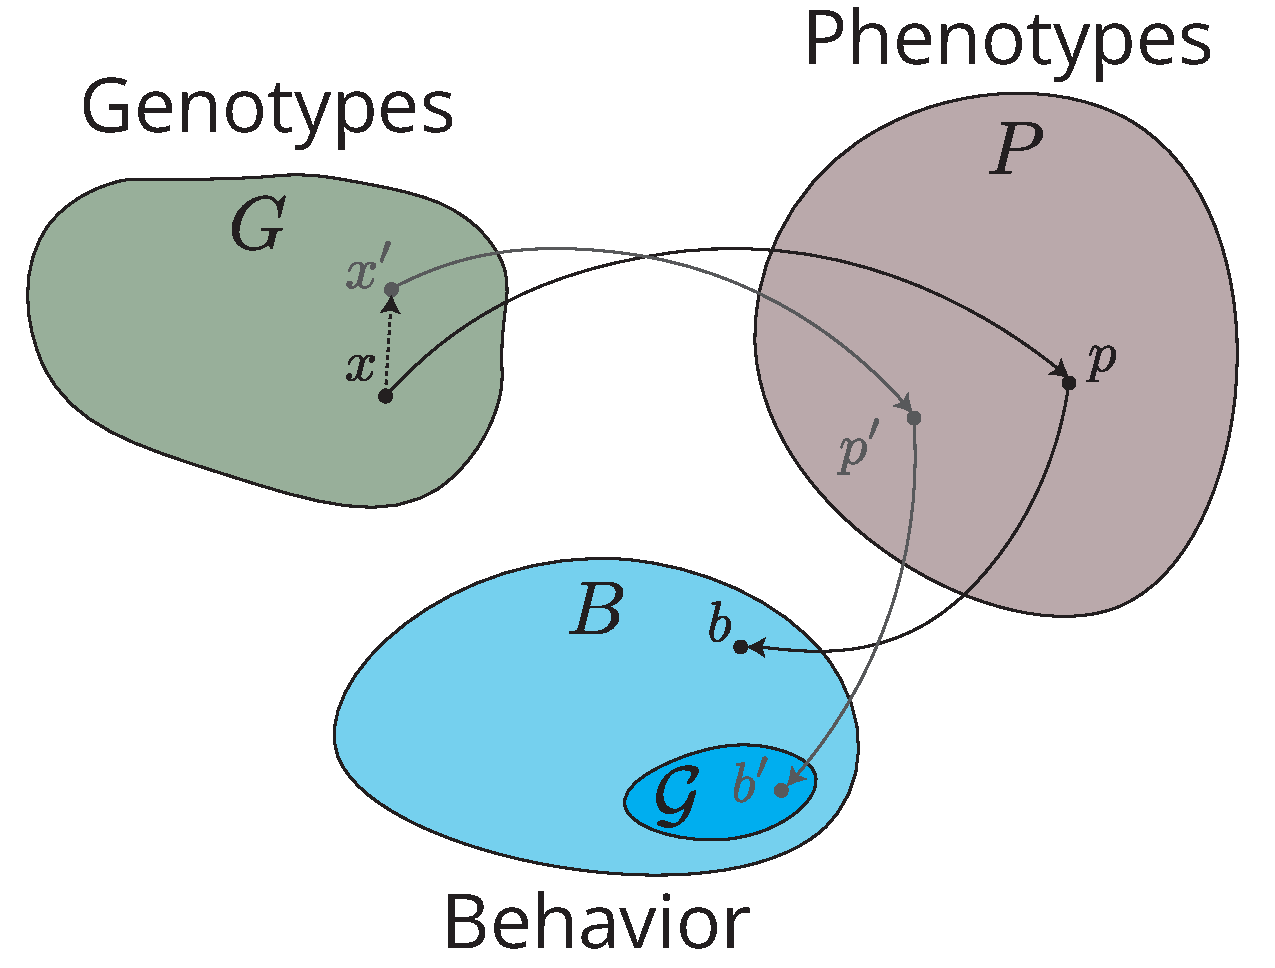
\includegraphics[width=.8\linewidth]{figures/evolutionary_diagram.pdf}
  \caption{Illustration of the general principle common to several evolutionary
    algorithms. There are three virtual spaces: ($G$) the genotype space where
    the candidate solutions are generated through some encoding. This is the
    space where the search process is happening. ($P$) the phenotype space,
    which corresponds to the decoded solution from a genotype $x$. It can be the
    policy of an agent, the rule of a \ac{CA}, etc. ($B$), the behavior space,
    which is the space from which candidate solutions are evaluated. The smaller
    subspace $\mathcal{G}$ is the goal space, corresponding to the set of
    behaviors that would be considered successful. A small perturbation in the
    genotype will have potentially large consequences on the behavior of the
    candidate solution. In the case of a \ac{CA} rule, the genotype could be a 
    vector ($x$) that encodes a rule ($p$) that will translate into the \ac{CA} behavior $b$.}
  \label{fig:evolutionary_diagram}
\end{figure}

\subsection{Genetic pr\label{sec:genetic-programming}ogramming}
Many of the problems that machine learning and artificial intelligence are
attempting to solve require the discovery of a computer program that produces
some desired mapping between inputs and outputs. Solving the problems therefore
amounts to searching the space of computer programs in order to find a suitable
individual with high enough fitness
\parencite{langdonFoundationsGeneticProgramming2002,
  kozaGeneticProgrammingMeans1994, banzhafGeneticProgrammingIntroduction1998,
  ,bookerClassifierSystemsGenetic1989}.

In genetic programming, candidate solutions to a problem are encoded as
\emph{chromosomes}, which is a structured data representation that can be
modified incrementally. In practice, it is often chosen to be a string of bits.
Every generation, a population of solutions is evaluated. The best solutions are
kept and combined to form the candidates for the next generation. Random
mutations may also be applied to introduce randomness in the search.

\subsection{Novelty search}
The idea behind \ac{NS} is to drive a search algorithm only by the novelty of
produced behavior \parencite{lehmanAbandoningObjectivesEvolution2011}. The most
counter-intuitive feature of this algorithm is that the actual objective of the
task is not taken into account at all during the search process. Generated
agents are evaluated solely on the novelty of their behavior. Despite this, it
appears to be at least as efficient as other search processes that are focused on goals, such as maze navigation and biped locomotion
\parencite{lehmanAbandoningObjectivesEvolution2011}, swarm robotics
\parencite{gomesEvolutionSwarmRobotics2013}, or neural network design
\parencite{risiEvolvingPlasticNeural2010}. \ac{NS} can lead to the discovery 
of innovative and creative solutions to complex and deceptive objectives that 
would be difficult or impossible to achieve using traditional optimization methods. 
We illustrate this property in Figure~\ref{fig:novelty_search}.

The principle of guiding search by novelty alone is closely related to the goal
of this thesis, and especially with the challenge of parametrizing and searching
the space of available complex systems without using any explicit goal function.
The purpose of \ac{NS} is to perform a search without a goal function, and we draw
inspiration from this algorithm throughout our work.

\begin{figure}[htbp]
  \centering
  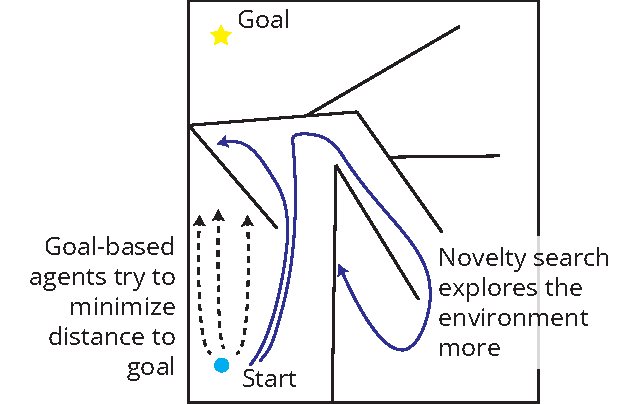
\includegraphics[width=.7\linewidth]{figures/novelty_search}
  \caption{Illustration of the advantage of \acf{NS} on a maze environment with
    deceptive dead-ends. Dotted trajectories illustrate the behavior of a
    goal-based search, which will start by minimizing the distance to the goal.
    Blue trajectories are from a novelty search algorithm exploring the space
    more efficiently. This type of maze environment was proposed by
    \textcite{lehmanAbandoningObjectivesEvolution2011}.}
\label{fig:novelty_search}
\end{figure}

This method has some limits, which are caused by a relative lack of theoretical
understanding of the effects of the parameters of \ac{NS}. The choice of
behavior descriptors for determining the novelty of agents is also not
straightforward. Several empirical studies have investigated the impact of a
range of parameters on the performance of \ac{NS}
\parencite{gomesDevisingEffectiveNovelty2015,
  kistemakerCriticalFactorsPerformance2011}, while other works have begun to
shed light on the theory \parencite{doncieuxNoveltySearchTheoretical2019}. In
practice \ac{NS} algorithms are expected to cover the exploration space well
\parencite{cullyQualityDiversityOptimization2017,pughQualityDiversityNew2016},
in some cases uniformly \parencite{gomesDevisingEffectiveNovelty2015}. \ac{NS}
algorithms are related to genetic algorithms since they maintain a population,
that is, a set of individuals used to measure the novelty of current solutions.
There is also an archive of the behavior of previous individuals to ensure that the
novelty is measured against all previously generated behaviors. There exists
multiple strategies for maintaining this archive
\parencite{gomesDevisingEffectiveNovelty2015}. Some use individuals whose
novelty was above a threshold when first evaluated
\parencite{lehmanAbandoningObjectivesEvolution2011}, the most novel individuals
of each generation \parencite{liapisConstrainedNoveltySearch2015}, random
individuals from the past generations
\parencite{lehmanEfficientlyEvolvingPrograms2010}, or none at all
\parencite{mouretEncouragingBehavioralDiversity2012}. An alternative to
explicitly measuring novelty in \ac{NS} is \emph{fitness sharing}. The goal of
fitness sharing is to encourage the diversity of a population by making them
share virtual ``resources'' \parencite{goldbergSimpleGeneticAlgorithms1987,
  hollandAdaptationNaturalArtificial1992}. A particular implementation of
\ac{NS} using this idea, with rewards physically spread across the
environment, was done by \textcite{herelEmergenceNoveltyEvolutionary2022}.

Typically, novelty search algorithms use one of a few types of maps from
genotypes to phenotypes, that is, a map from the space of encoded solution to
agent and policy implementation
\parencite{mouretEncouragingBehavioralDiversity2012}. Some common ones are:

\begin{itemize}
  \item A \ac{RNN} (of type \cite{elmanFindingStructureTime1990} or
        \cite{jordanSerialOrderParallel1997}), for which the weights are
        directly searched. For input size $n_{i}$ output size $n_{o}$, and
        hidden size $n_{h}$, $n_{i}n_{h} + n_{h}n_{o} + n_{h}^{2}$ weights must
        be evolved.
  \item Neuro-evolution of augmenting topology (NEAT,
        \cite{stanleyEvolvingNeuralNetworks2002}), which is an encoding of both
        neural network weights and architectures that has a built-in mechanism
        to sustain diversity.
\end{itemize}


\section{Open-ended evolution\label{sec:open-ended-evolution-1}}
The field of Artificial Life research has worked to figure out what the
fundamental conditions for the emergence of living systems are, and how to
create a process that can display analogous levels of creativity and complexity
as natural evolution \parencite{eigenHypercycle1979,
  langtonArtificialLifeProceedings1989, dysonOriginsLife1999,
  stanleyWhyOpenEndednessMatters2019, packardOverviewOpenEndedEvolution2019,
  sorosOpenendednessLastGrand2017}. It builds upon the data and understanding we
collected about the process of life, but abstracts from any specific living
process and attempts to integrate various approaches into one unified research
to extract the first principles of life. A major assumption underpinning this
research is that this natural evolutionary process can be implemented equally
well in different media \parencite{dennettDarwinDangerousIdea1996}.

A system that behaves like natural evolution, producing a seemingly endless
amount of novelty and complexity starting from elementary building blocks is
called \emph{open-ended}. The main challenge of \ac{OEE} research is that there is
no single simple test for the phenomenon, but instead different kinds of
open-ended evolution exist. Systems can exhibit more than one kind at a time. In
the report from a workshop on \ac{OEE} at York
\parencite{taylorOpenEndedEvolutionPerspectives2016}, the authors summarized the
different types of \ac{OEE}, which were further refined in a follow-up work
\parencite{packardOverviewOpenEndedEvolution2019}. They are:

\begin{enumerate}
  \item Interesting new kinds of entities and interactions
  \item Evolution of evolvability
  \item Major transitions
  \item Semantic evolution.
\end{enumerate}

The first category describes the ability of a system to construct new entities
with different properties, behaviors, or interactions with other entities. For
example, the Tierra simulation sees entities emerge that exploit the computing
power of others, acting as parasites \parencite{rayApproachSynthesisLife1991}.
The second type is related to how open-ended evolution itself can be evolved
through the emergence of multiple ``stepping stones'' that allow individuals to use higher-level evolutionary units or through interactions
\parencite{patteeEvolvedOpenEndednessNot2019}. ``Major transitions'' refer to
the emergence of new levels of hierarchy in evolving populations. These
transitions are characterized by groups of reproducing entities that
interact tightly and form a new population of higher-level reproducing entities.
The process can repeat, with certain groups in the new population forming even
higher-level entities. This process of emergence of major transitions was
explored in \parencite{sayamaCardinalityLeapOpenEnded2019,
  morenoOpenEndedFraternalTransitions2019} for example. Lastly, semantic
evolution is related to the work of
\textcite{ikegamiOpenEndedEvolutionMechanism2019}, who propose a new category of
open-ended evolution called semantic evolution, which refers to the evolution of
semantic relationships within a system. This can be observed in the evolution of
web services, where the meaning of tags changes as new combinations of tags are
created. It is not biological in nature and is also present in the analysis of
technological evolution \parencite{bedauOpenEndedTechnologicalInnovation2019},
where the meaning and importance of keywords shift over time.

\subsection{Defining open-endedness}

Several necessary conditions and requirements have been identified in the
\ac{OEE} literature, forming an overlapping set of potential research
directions for developing open-ended systems. We list a few of these conditions
here. First, \textcite{maleyFourStepsOpenended1999} identifies four requirements:

\begin{enumerate}
  \item An open-ended evolutionary system must demonstrate unbounded diversity
        during its growth phase.
  \item An open-ended evolutionary system must embody selection.
  \item An open-ended evolutionary system must exhibit continuing new adaptive
        activity.
  \item An open-ended evolutionary system must have an endogenous implementation
        of niches.
\end{enumerate}
Next, \textcite{sorosIdentifyingNecessaryConditions2014} identified four more necessary
conditions, which are

\begin{enumerate}
  \item A rule should be enforced that individuals must meet some minimal
        criterion (MC) before they can reproduce, and that criterion must be
        nontrivial.
  \item The evolution of new individuals should create novel opportunities for
        satisfying the MC.
  \item Decisions about how and where individuals interact with the world should
        be made by the individuals themselves.
  \item The potential size and complexity of the individuals' phenotypes should
        be (in principle) unbounded.
\end{enumerate}
Then, \textcite{taylorRequirementsOpenEndedEvolution2015} also stated five
requirements for an open-ended system:

\begin{enumerate}
  \item Robustly reproductive individuals.
  \item A medium allowing the possible existence of a practically unlimited
        diversity of individuals and interactions, at various levels of
        complexity.
  \item Individuals capable of producing more complex offspring.
  \item An evolutionary search space that typically offers mutational pathways
        from one viable individual to another viable (and potentially fitter )
        individuals.
  \item Drive for continued evolution.
\end{enumerate}
Taylor also states a more general condition that should be sufficient for
creating an open-ended system as ``evolutionary dynamics in which new,
surprising, and sometimes more complex organisms continue to appear''
\parencite{taylorRequirementsOpenEndedEvolution2015,
  taylorOpenEndedEvolutionPerspectives2016}.

All these conditions illustrate a major challenge of \ac{OEE} research: the lack
of a clear definition or notion of what exact conditions make a system
open-ended. We seem to agree about what is not open-ended, but whenever a
constraint or requirement for \ac{OEE} is identified, subsequent evidence forces
us to refine them later. This is related to the problem of complexity, for which
no single definition exists \parencite{johnsonSimplyComplexityClear2009}.

A common process to produce systems that behave analogously to natural evolution
is to start from evolvable units or building blocks
\parencite{rayApproachSynthesisLife1991, simsEvolvingVirtualCreatures1994,
  ofriaAvidaSoftwarePlatform2004, yaegerComputationalGeneticsPhysiology1994,
  channonImprovingStillPassing2003, spectorDivisionBlocksOpenended2007,
  sorosIdentifyingNecessaryConditions2014}. The reason is that starting from
higher-level primitive units whose emergence would be hard to characterize may
be easier and faster than starting from lower-level components. The results obtained
from these systems are often surprising, as they bear some key similarities
to natural evolutionary processes. For example, we note the emergence of
parasitic entities within the Tierra simulation
\parencite{rayApproachSynthesisLife1991}. The process of emergence of these
building blocks from simple rules and components has also been investigated
significantly \parencite{bagleySpontaneousEmergenceMetabolism1991,
  huttonEvolvableSelfReproducingCells2007, flammEvolutionMetabolicNetworks2010,
  sayamaSeekingOpenendedEvolution2011}. It appears harder to bridge the gap and
create high-level evolutionary-like processes and behaviors from elementary
rules and substrates.

\subsection{Open-endedness in cellular automata}
One class of systems that has rich interactions between each of its components, as
well as no predefined evolvable units or assumptions about individuality is the
\ac{CA}. One of the very first automata, Von Neumann's self-reproducing machine,
was designed with goals that align with open-ended evolution, which is to build
a machine with no central controller and limited local interaction that can
self-reproduce as a whole
\parencite{vonneumannTheorySelfreproducingAutomata1966,
  pesaventoImplementationNeumannSelfReproducing1995}. Later, other
self-replicating structures such as Langton's loop
\parencite{langtonSelfreproductionCellularAutomata1984} and evoloops
\parencite{sayamaNewStructurallyDissolvable1999,
  salzbergComplexGeneticEvolution2004} showed that more properties of open-ended
systems can be included in a \ac{CA}. A potential limitation of \acp{CA} is the
absence of the notion of conservation of ``matter''. For example, the game of life
can start from a configuration with very few live cells and create many more at
no cost during its evolution. Some authors believe that this conservation
property is essential to the construction of an open-ended evolving system
\parencite{taylorChapterCreativityEvolution2002}.

\subsection{Artificial chemistries}
Artificial chemistries, are computational models that aim to simulate the
behavior of chemical systems, which are typically used to study the emergence of
complex behavior from simple interactions between individual molecules. Most of
the time, \acp{AC} do not try to accurately model chemical processes (as in
\parencite{ostrovskyCellularAutomataPolymer2001,
  buligaChemlambdaUniversalitySelfmultiplication2014,
  bedauLessAbstractArtificial2000, sayamaSeekingOpenendedEvolution2011} for
example). Instead, they build models of the dynamics of complex molecular
processes that lead to evolutionary behavior
\parencite{dittrichArtificialChemistriesReview2001}. By abstracting away from natural molecular processes, \acp{AC} tries to uncover fundamental
conditions for the emergence of organization, self-maintenance, or
self-construction with basic building blocks. There are various approaches for
building these \aclp{AC}, of which we review a few here.

\paragraph{Rewriting systems.}
Rewriting systems are a class of computational models that use a set of
rewriting rules to transform and manipulate strings of symbols. They are
composed of entities or symbols that get modified according to their set of
syntactic rules. Patterns of symbols or entities are replaced according to these
rules. In AlChemy \parencite{fontanaWhatWouldBe1994}, molecules are represented
as expressions in the $\lambda$-calculus. The $\lambda$-calculus is a mathematical formalism
that, like Turing machines, is capable of describing any computable function. In
AlChemy, pairs of randomly selected expressions are joined using function
application, evaluated, and the resulting value is added back to the population
of molecules. This process is repeated to simulate the behavior of a chemical
system. \textcite{kruszewskiEmergenceSelfReproducingMetabolisms2022}
hypothesized that self-reproducing metabolisms emerge as a subset of
autocatalyzed reactions within a Turing-complete set. They introduced
\emph{combinatory chemistry}, an artificial chemistry designed to capture the
core computational properties of living systems that is based on the rewriting
rules of \emph{combinatory logic} \parencite{curryCombinatoryLogic1958,
  schoenfinkelUeberBausteineMathematischen1924}. The generated structures
exhibit behaviors that are similar to natural metabolisms. The system is able to
represent patterns of arbitrary complexity, and it is able to produce diverse
self-reproducing patterns.

\paragraph{Cellular automata.}
\Acfp{CA} can be seen as a particular case of lattice molecular systems. For
example, the autopoietic system (referring to the ability of an organism to continuously 
sustain itself through the exchange of matter and energy with its environment, 
while maintaining its own boundaries and identity) introduced by
\textcite{varelaAutopoiesisOrganizationLiving1991} is a 2D square grid with
sites that be occupied by \emph{atoms} which is similar to a \ac{CA} with 4
states. Each of these states is analogous to a chemical component of the system:
($\emptyset$) empty site, (S) substrate, (K) catalyst, and (L) monomer. Basic rules are
applied asynchronously and define how neighboring atoms interact with each
other. Remarkably, stable self-repairing cells spontaneously arise from these
basic rules. Their membrane is composed of a chain of monomers, which is
maintained by the substrate and catalyst reacting according to the rules. Some
key components of that model were investigated in other works, showing that they
are crucial for this emergence autopoeisis to be possible
\parencite{zelenySelforganizationLivingSystems1977,
  mcmullinRediscoveringComputationalAutopoiesis1997}.

\section{Computing with complex systems}\label{sec:comp-with-compl}

The problem of computing within complex systems is closely related to the
question of decentralized parallel computation, in general, for which there exists
abundant literature. Different paradigms exist for controlling and harvesting
the computations within complex systems. Several other names have been used for
closely related topics, such as organic computing
\parencite{muller-schloerOrganicComputingParadigm2011} which is the study of
systems with life-like properties such as self-organization or the ability to
adapt to a dynamically changing environment. Agent-based computing
\parencite{jenningsAgentBasedComputingPromise1999} focuses on computing systems
composed of several relatively simple autonomous agents. Amorphous computing
\parencite{abelsonAmorphousComputing2000,
  nagpalProgrammablePatternFormationScaleIndependence2008,
  nagpalProgrammableSelfassemblyUsing2002} is about making large amounts of
individual computing elements work and ensuring ``the cooperation of large
numbers of unreliable parts interconnected in unknown, irregular, and
time-varying ways''.

\subsection{Computing in cellular automata}\label{sec:comp-cell-autom}

\Acfp{CA} are decentralized parallel systems with many identical components with
local connectivity. Because of these properties, they have the potential to
carry out robust and efficient computations. \ac{CA}-based computing machines could
recover from perturbations or carry out computations in stochastic environments.
Moreover, they are also interesting for modeling the behavior of natural complex
systems. For more details on \acp{CA}, see Section~\ref{sec:cellular-automata-sec}.

\paragraph{Von Neumann's self-reproducing \ac{CA}.}
The early developments of \acp{CA} were guided by Von Neumann's question ``What
kind of logical organization is sufficient for an automaton to be able to
reproduce itself?'' Since this question may admit very simple solutions,
additional constraints were added so that the problem does not admit trivial
solutions. For example, Von Neumann required that the automaton in question be
equivalent in power to a universal Turing machine while having minimal
complexity \parencite{vonneumannTheorySelfreproducingAutomata1966}. The final
model he proposed was an intricate \ac{CA} composed of a tape containing the
instructions to construct the next automaton and a construction unit that
would progressively build that new automaton cell by cell. This was an early
example of complex computations being carried out by a relatively simple
decentralized system such as a \ac{CA}.

\paragraph{Universal Computation in Cellular Automata.}
It is not difficult to see that a \ac{CA} can be capable of universal
computation. The basic approach is to show that it can simulate a Turing
machine, which we assume has an infinite tape. A \ac{CA} rule can be constructed
by reproducing all the steps of a Turing machine's behavior while adding a state
to each cell, indicating whether it is active or not, and enforcing that only one
cell is active at a time. This turns the parallel \ac{CA} into a sequential
object that simulates a Turing machine. A similar construction was carried out
by \parencite{smithSimpleComputationUniversalCellular1971}, making a \ac{CA}
with one-to-one correspondence between its time steps and that of a target
Turing machine.

Another approach was used to show the universality of the game of life (see
details in Section \ref{sec:game-life}). Instead of simulating a Turing machine,
basic logical functions are built from gliders (see figure \ref{fig:glider})
produced by a game of life structure called \emph{glider gun}. Two gliders that
collide within the simulation will either annihilate or keep moving depending on
the exact position in which they collide. This allows the construction of NOT, AND and
OR gates. For example, see Figure \ref{fig:gol_not_gate} for a construction of a
NOT gate in the game of life.

\begin{figure}[htbp]
  \centering
  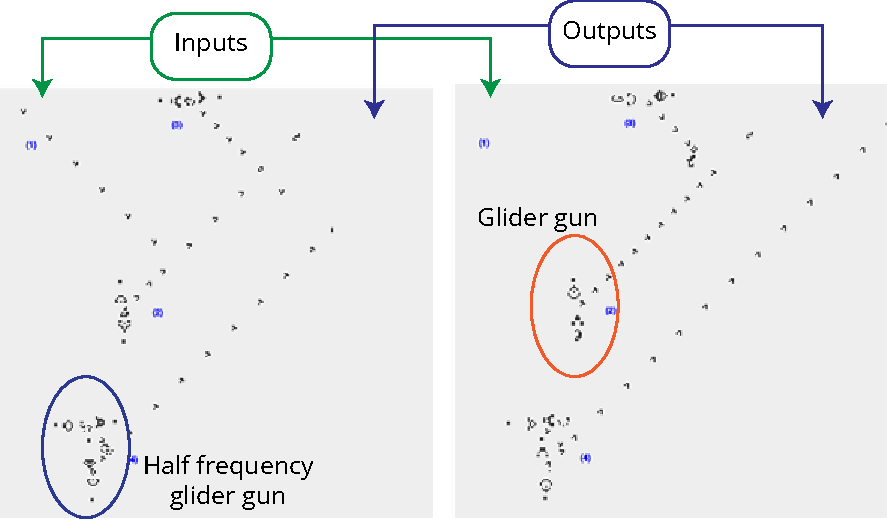
\includegraphics[width=.8\linewidth]{figures/gol_not_gate}
  \caption{Construction of a NOT gate in game of life. The left image represents
    an input equal to 1, while the second shows an input equal to 0. Output
    streams behave like a NOT gate. A glider gun and a modified half-frequency
    glider gun are highlighted. They are necessary for the construction of the
    gate. Images are adapted from a blog post
    \parencite{carliniDigitalLogicGates2020}.}
  \label{fig:gol_not_gate}
\end{figure}

Universal computation is an intriguing yet impractical property, and proving
that a system is a universal computers often has limited usability, but it
serves as a proof of principle that the studied system is theoretically as
powerful as any computer. In the case of the game of life, this was illustrated
by the implementation of the OTCA metapixel which is a tileable square cell
object that can be used to simulate another instance of game of life within the
game. It is important to note that such embedded computers and Turing machines
are often very slow and inefficient, and the game of life has brittle structures
which would be destroyed by the slightest perturbation, making these
constructions unusable for anything else than demonstration.

\paragraph{Evolving cellular automata with genetic algorithms.}
An important advancement beyond the clever yet challenging manual design of 
computational rules in \acp{CA} is the utilization of learning algorithms 
for automated rule design \parencite{mitchellEvolvingCellularAutomata1996}. 
Genetic algorithms, which are search methods inspired 
by biological evolution, are one such type of
learning algorithm \parencite{bookerClassifierSystemsGenetic1989}. See Section
\ref{sec:genetic-programming} for more details about genetic algorithms.

Some early work on evolving \acp{CA} was done by Norman Packard and colleagues
\parencite{packardAdaptationEdgeChaos1988,
  richardsExtractingCellularAutomaton1990}.
\textcite{richardsExtractingCellularAutomaton1990} used genetic algorithms to
learn the rules of \ac{CA} to match experimental data for the patterns created
by dendritic solidification of \ce{NH4Br}. In
\parencite{packardAdaptationEdgeChaos1988}, the author evolves \acp{CA} to
perform a specific computation, and observes that the evolution process tends to
select \acp{CA} with a $\lambda$ parameter close to the critical value observed by
Langton that corresponds to the edge of chaos (see Section
\ref{sec:langtons-lambda} for details about the parameter). However, other
authors were unable to replicate this experiment later
\parencite{mitchellRevisitingEdgeChaos1993}.
\textcite{kozaEvolutionSubsumptionUsing1992} applied genetic algorithms to
\acp{CA} to generate random numbers.

The problem of density classification was thoroughly explored since it fits the
\ac{CA} paradigm particularly well \parencite{mitchellRevisitingEdgeChaos1993,
  mitchellEvolvingCellularAutomata1994,
  crutchfieldEvolutionEmergentComputation1995, dasGeneticAlgorithmDiscovers1994,
  sipperCoevolvingNonuniformCellular1996, andreDiscoveryGeneticProgramming1996}.
The goal of this task is to have \acp{CA} figure out what the most abundant cell
state in an initial binary configuration in one dimension is. This task is trivial
for a central controller that can read the state of all cells in the initial
grid, but it is much more complex for decentralized systems like \acp{CA}
that have a small radius of interaction with neighbors. The evolved \acp{CA}
developed various strategies to solve the task. Some are unsophisticated, such
as expanding the 1s or 0s, which does not work on all validation examples. We
show one of the more sophisticated solutions discovered during some runs of the
genetic algorithm in figure \ref{fig:particle_ca}. That solution uses the
propagation of structures within the \ac{CA} state space to communicate the
local state to the rest of the grid, which usually ends with the right answer
from the \ac{CA}.

\begin{figure}[htbp]
  \centering
  \begin{subfigure}[b]{.4\linewidth}
    \centering
    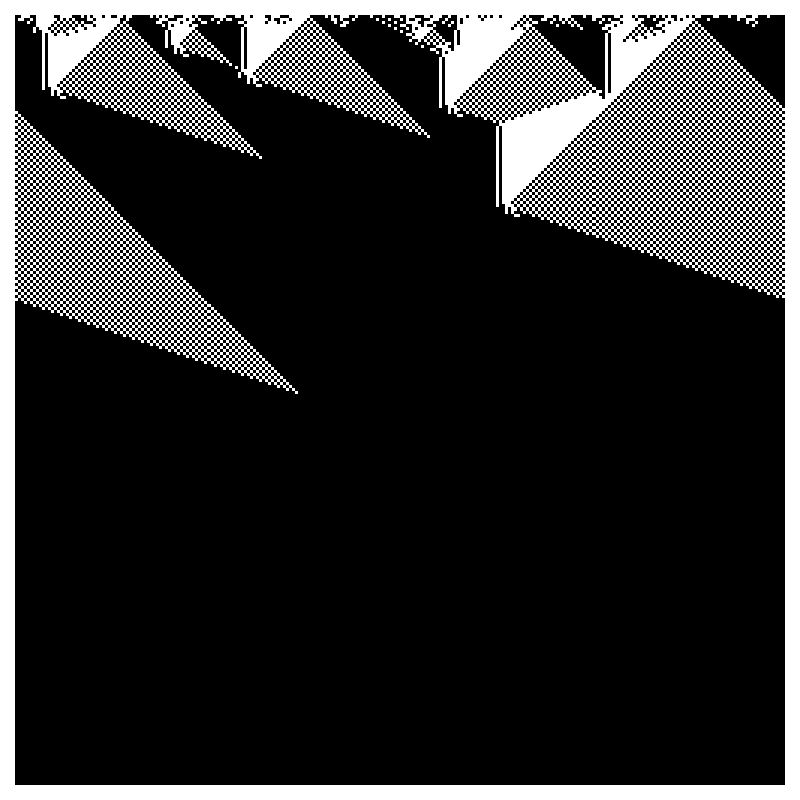
\includegraphics[width=\linewidth]{figures/particle_ca_full.png}
    \caption{Density $> 0.5$}
    \label{fig:particle_ca_full}
  \end{subfigure}
  \hspace{10pt}
  \begin{subfigure}[b]{.4\linewidth}
    \centering
    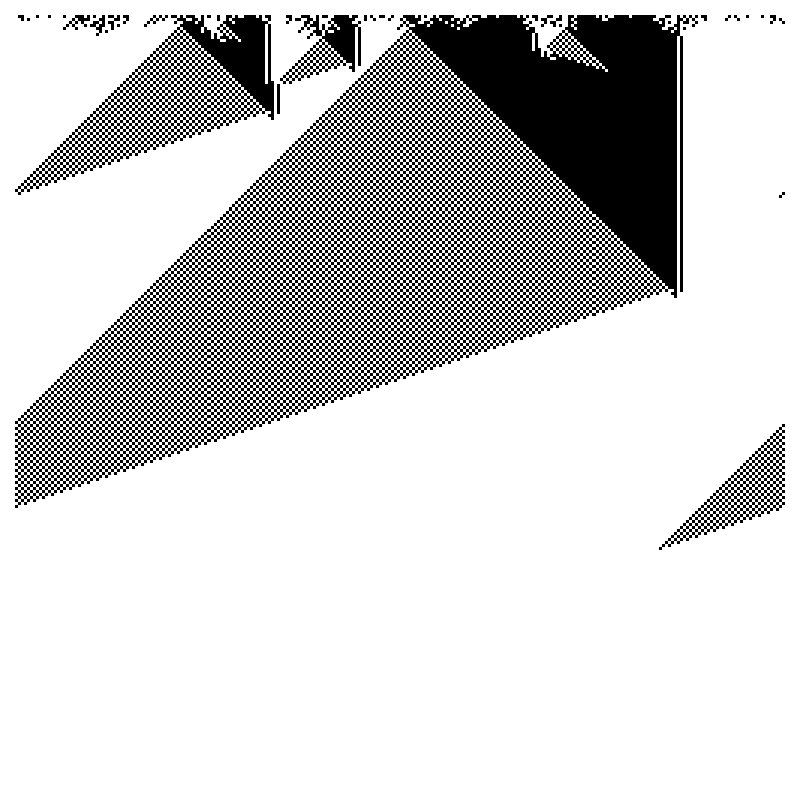
\includegraphics[width=\linewidth]{figures/particle_ca_empty.png}
    \caption{Density $< 0.5$}
    \label{fig:particle_ca_empty}
  \end{subfigure}
  \caption{The particule-based solution to the density classification problem
    \parencite{mitchellEvolvingCellularAutomata1996}. When the density is above
    0.5, the \ac{CA} quickly reaches a state with only black cells, whereas when
    the density is lower, it goes to a state with white cells only.}
  \label{fig:particle_ca}
\end{figure}


\paragraph{Reliable computation in cellular automata.}
The problem of carrying out reliable computations in \acp{CA} is studied early
on in its history because of the potential of that model for a real hardware
implementation. The first studies used probabilistic approaches for solving the
error detection and correction problems of automata --- which includes other
models than \acp{CA} \parencite{neumannProbabilisticLogicsSynthesis1956,
  winogradReliableComputationPresence1963,
  ,tsertsvadzeStochasticAutomataProblem1964,
  ,haraoConsiderationCellularAutomata1973}. Other methods make use of the
special structure of \acp{CA}, but rely on strong assumptions about the
likelihood of errors \parencite{haraoFaultTolerantCellular1975,
  nishioFaultTolerantCellular1975}. Peter Gács has shown how to construct a 1D
\ac{CA} which can perform arbitrarily large reliable computations, assuming that each
cell gets an error with a positive probability
\parencite{gacsReliableComputationCellular1986}. The fault model he describes is
important from the point of view of ergodic theory because Gács’ result
invalidates the ``positive probability conjecture'' in statistical physics,
which states that all one dimensional infinite particle systems with positive
transition probabilities are ergodic, which means that it will visit all parts of
its state space eventually. For more recent work on fault tolerance by Gács, see
\parencite{gacsReliableCellularAutomata2001}.

\paragraph{Neural cellular automata\label{sec:neur-cell-autom}.}
The principle of \ac{NCA} is based on the analogy between \acp{CA} and two types
of neural networks: \acp{RNN} and \acp{CNN} (see Section
\ref{sec:cell-autom-rnns} for more details about the analogy). Following this
analogy, \acp{CA} can be formulated as a continuous recurrent and convolutional
neural network system called a \acf{NCA}. \acp{NCA} can be manipulated like
neural networks, using automatic differentiation, backpropagation, and
optimization algorithms to make these models learn some target task. The first
example used this neural network representation to learn a \ac{NCA} version of
existing \ac{CA} rules from recorded examples of their evolution
\parencite{gilpinCellularAutomataConvolutional2018}. The structure of the
training process and the final error of the resulting model are used by the author as
a tool to understand the complexity and properties of the original \ac{CA}.

\acp{NCA} were also used to learn to produce stable self-repairing patterns that
resemble a target image \parencite{mordvintsevGrowingNeuralCellular2020}. The
training process is structured in such a way that the \ac{NCA} needs to learn to
maintain the pattern stable across time and space, but also recover form random
perturbations that are introduced at arbitrary points in time. This results in
an interesting demo where a pattern is generated and maintained in real-time by
a \ac{NCA} while a user can directly apply
perturbations\footnote{\url{https://distill.pub/2020/growing-ca/}}.

\begin{figure}[htbp]
  \centering
  \begin{subfigure}[t]{.49\linewidth}
    \centering
    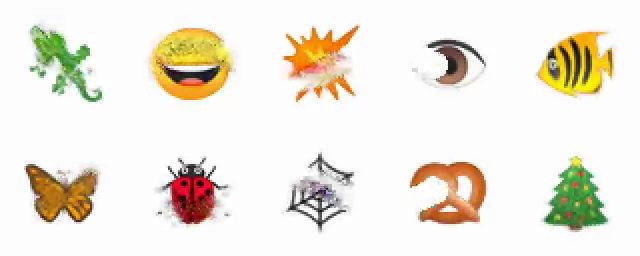
\includegraphics[width=\linewidth]{figures/nca_perturb.png}
    \caption{Perturbed patterns}
    \label{fig:nca_perturb}
  \end{subfigure}
  \begin{subfigure}[t]{.49\linewidth}
    \centering
    
\includegraphics[width=\linewidth]{figures/nca_recover.png}
    \caption{Recovered patterns after a few hundred \ac{NCA} steps.}
    \label{fig:nca_recover}
  \end{subfigure}
  \caption[Resistance of patterns]{Resistance of patterns to perturbations with
    \acp{NCA}. \ac{NCA} can robustly maintain patterns, even under relatively
    strong perturbations (~10-20\% of the pattern's size). This image was
    generated with an online notebook based on code from Alexander
    Mordvintsev\footnotemark.}
  \label{fig:nca}
\end{figure}
\footnotetext{\url{https://colab.research.google.com/github/google-research/self-organising-systems/blob/master/notebooks/growing_ca.ipynb}}

The same authors also used \acp{NCA} to learn to classify digits from the MNIST
database of handwritten digits
\parencite{randazzoSelfclassifyingMNISTDigits2020}. The particularity of this
model is its ability to perform the classification in a decentralized way, by
having the \ac{NCA} change the color of the digits directly on the \ac{CA} grid.
Cells can only communicate with their direct neighbors, so the model has to
reach a consensus by spreading information across the grid. This is done in
parallel, so multiple digits can be classified simultaneously through this
progressive consensus
process\footnote{\url{https://distill.pub/2020/selforg/mnist/}}.
Another work used the same model to learn to continuously generate images with
the same texture as a target \parencite{niklassonSelfOrganisingTextures2021}.
Again, an advantage of this method is the ability to recover from perturbations.

\begin{figure}[htbp]
  \centering
  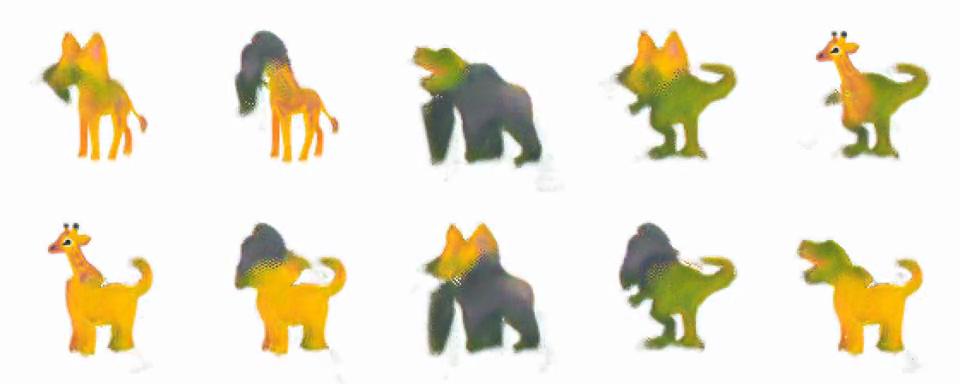
\includegraphics[width=.8\linewidth]{figures/nca_hybrids.png}
  \caption{Examples of stable hybrids obtained with \acp{NCA} trained with the
    method of \parencite{cisnerosOpenendedCreationHybrid2021}.}
  \label{fig:nca_hybrid}
\end{figure}


We used \acp{NCA} as part of our submission to the Minecraft open-endedness
challenge 2021\footnote{\url{https://evocraft.life/}}, a competition organized
at the Gecco 2021 conference competition
track\footnote{\url{https://gecco-2021.sigevo.org/Competitions}}
\parencite{cisnerosOpenendedCreationHybrid2021}. The goal was to build an
open-ended system within the computer game Minecraft. This means building a
systems that fulfill the following requirements:

\begin{itemize}
  \item Divergence: Open-ended algorithms are not expected to slow down or
        converge but rather keep expanding and generating more complex outputs
        over time.

  \item Diversity: Does the algorithm produce entities with strong phenotypic
        diversity?

  \item Complexity: Can the algorithm produce complex entities or entities
        interactions that give rise to complex systems? Are hierarchical and
        modular structures present?

  \item Ecological interactions: Do the created entities interact with each
        other?

  \item Life-Like properties: Inspiration may be taken from other attributes of
        living systems.
\end{itemize}

In each of the examples in Figure \ref{fig:nca}, a separate \ac{CA} was trained
on a pattern starting from a single black pixel. We extend this setup by
training a single \ac{NCA} on multiple patterns from different seeds. Instead of
a single black cell, a small number of black cells are arranged in simple
shapes. We call these patterns \emph{seeds}. \acp{NCA} are neural networks with many redundant parameters. This allowed us to learn (and encode) more than one
pattern (or larger patterns) without adding parameters in the architecture. The
resulting patterns are slightly lower quality but still stable under
perturbations and capable of growing from their corresponding seed pattern.

We turned the process of combining seed patterns into a ``game'' by allowing user
interaction with the evolving CA through the Minecraft video game, using an API
to communicate between the program and the game. Our system is not open-ended by
itself, but serves as an exploration space and uses human interactions to play
with the shapes and seed patterns. This is in the spirit of open-ended game-like
systems like Picbreeder \parencite{secretanPicbreederCaseStudy2011,
  woolleyDeleteriousEffectsPriori2011} where players choose which generated
image to mutate or evolve from, collectively constructing surprisingly complex
images. The algorithms can generate endless novelty with the help of human
interactions that provide the missing step for making the system potentially
open-ended.

\subsection{Amorphous computing}
The goal of amorphous computing is to study and define the problem of computing
with multiple interconnected components that are unreliable, irregular,
time-varying, and with limited computational capacity
\parencite{abelsonAmorphousComputing2000}. The motivation for this area of
research is the development of biological substrates that can compute, function
as sensors and actuators, and robustly self-organize to compute with little
cost. The precise manufacturing of chemical or biological substrates with the ability
to communicate locally through chemical or physical interactions is within
reach, making their use as computing vessels particularly
attractive. We can embed millions of chips with sensors
\parencite{abelsonAmorphousComputing2000} or program biological cells to serve
as logic gates \parencite{weissProgrammingBiologicalCells1998,
  weissVivoDigitalCircuits2002} while relying on cheaper, decentralized parts
\parencite{buteraProgrammingPaintableComputer2002}.

\begin{figure}[htbp]
  \centering
  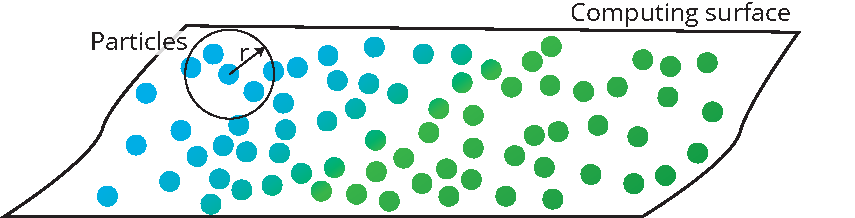
\includegraphics[width=.8\linewidth]{figures/amorphous_computing}
  \caption{An example of amorphous computing on a surface. Multiple computing
    particles are arranged randomly. A wave (represented by the color of the
    cells) propagates within the medium. They can communicate with neighbors
    within a radius $r$.}
  \label{fig:amorphous_computing}
\end{figure}

In amorphous computing systems, a medium comprises ``computational
particles'' spread on a surface or mixed in a volume. The particles have 
limited computing power, with no knowledge of their position or orientation. The
particles can communicate with neighbors via some specified mechanism, which may
be analogous to biological ones. The two main components of this research are 
\emph{synthetic biology} and the choice of computing paradigm.
\begin{description}
  \item[Synthetic biology.] The design of a substrate from chemical processes or
        genetically engineered biological cells
        \parencite{weissVivoDigitalCircuits2002}. It should behave correctly and
        follow predefined rules.
  \item[Computing paradigm.] How to program individual agents to follow a
        predefined global goal
        \parencite{nagpalProgrammableSelfassemblyConstructing2001}?
\end{description}


The growing point language (GPL) is an example of a programming language that
enables programmers to specify complex patterns for computational particles,
which are internally represented in the particles as state machines
\parencite{cooreBotanicalComputingDevelopmental1999}.

\textcite{nagpalProgrammableSelfassemblyUsing2002} developed another
programming language inspired by biological cell differentiation
\parencite{lawrenceMakingFlyGenetics1992,
  wolpertPositionalInformationSpatial1969} that can be compiled into individual agent
programs to follow some global specifications.
